\chapter{Bitcoin Attacks}

Naive attempts to \textbf{double spending} are easily detected and rejected by the network.
By sending two transactions that spend the same coin, the network will accept only one of them, the first one that arrives. The second transaction will be rejected as it tries to spend a coin that has already been spent.
Or, still, adding the same coin two times in the same block will be rejected by the network, as the block would be invalid.\\
However, there are more sophisticated attacks that can be performed on the Bitcoin network. Later on in this chapter we will discuss some of them.

\section{Forks}
If two blocks $A$ and $B$ are mined at the same time (actually, the second is mined before the first is propagated through the network), the network will have two different versions of the blockchain. This is called a fork.
\begin{paracol}{2}
   \colfill	
   \begin{figure}[htbp]
      \centering
      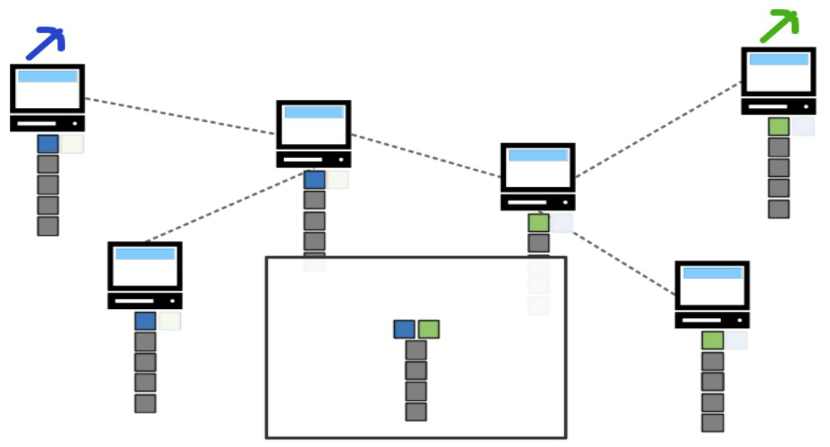
\includegraphics{images/bitcoin_fork.png}
      \caption{Bitcoin Fork}
      \label{fig:bitcoin_fork}
   \end{figure}
   \colfill
   \switchcolumn
   Some nodes will have $A$ as the last block, and some others will have $B$. 
   The two versions will \textit{coexist} until the next block is mined: if the next block is mined on top of $A$, then such chain becomes the longest and the network will accept it as the main chain, and the $B$ chain will be discarded, requiring a slight reorganization of the chain. This applies specularly if the next block is mined on top of $B$.
\end{paracol}

\framedt{Forks and double spending}{
   If an attacker performs a double spending attack by sending two transactions that spend the same coin, typically one of the two will be mined before the other (they cannot coexist in the same block), and the latter will result invalid and never mined by nodes.
   But it may happen that the two transactions are mined simultaneously in two different blocks, resulting in a \textbf{fork}. To avoid so, \ul{a transaction is accepted by the network only after 6 blocks have been mined on top of it} (Def. \ref{def:6confirmation}).
}

\newpage
\section{51\% Attack}
\label{sec:51-attack}
\begin{paracol}{2}
   \colfill
   This attacks addresses the double spending problem by controlling the majority of the network's mining power.
   The attacker can then create a ``hidden'' fork of the\\ blockchain,
   where the transaction that he wants to double spend is not included.
   He avoid broadcasting its fork until his chain is longer than the main chain, where he had spent its coins. At that point, he can broadcast his fork ---where he still owns its Bitcoins!--- and the network will accept it as the longest chain.
   \colfill
   \switchcolumn

   \begin{figure}[htbp]
      \centering
      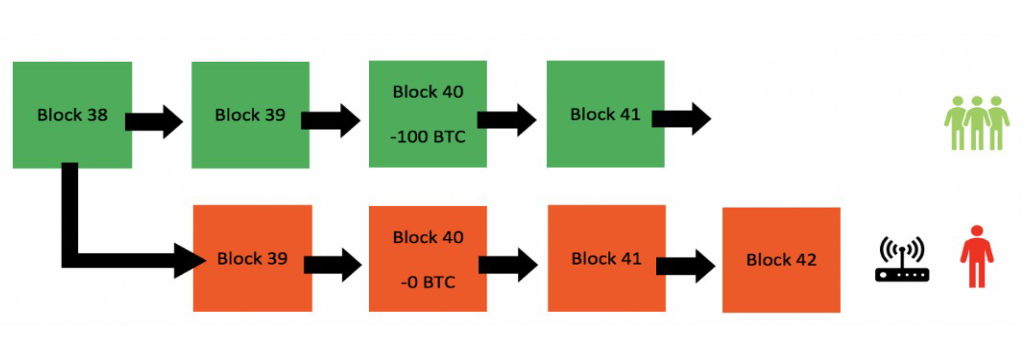
\includegraphics{images/bitcoin_atk511.png}\\
      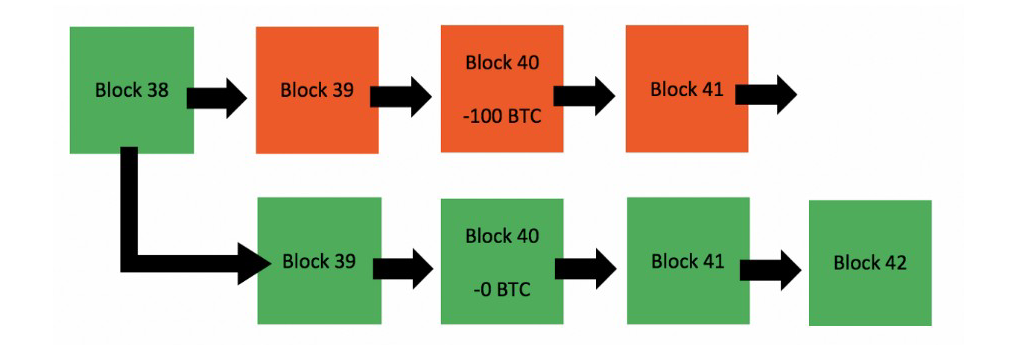
\includegraphics{images/bitcoin_atk512.png}
      \caption{Bitcoin 51\% Attack}
      \label{fig:bitcoin_atk51}
   \end{figure}
\end{paracol}

This attack requires for the attacker to control more than 50\% of the whole network's mining power, which is a \textit{very difficult} task. It is pretty unlikely that an attacker succeeds.

In 2014 \texttt{GHash.io}, a mining pool, reached 51\% of the network's mining power. The pool was asked to reduce its power, and it did.

\section{Transaction Malleability}
A subtle attack on the Bitcoin network is the transaction malleability. This attack does not allow to double spend, but it can be used to confuse the network and the users.

Recall that the transaction inputs are signed with the private key of the owners of the funds, allowing to verify the ownership of the funds.
All the nodes receiving a transaction verify that the sender(s) are really the owners of the transaction.

A node can change the unlocking script in such a way that the transaction has the same effect and the signature is still valid, but the \textit{TXID changes!}
The transaction ID \ul{TXID is computed by hashing a set of data that is a superset of the fields covered by the signature}.
Adding a \texttt{NO\_OP} operation in the unlocking script, or changing the order of the operations, will change the TXID, but the signature and the unlocking script will still be valid.

\subsection{Exploiting Malleability}
\texttt{Alice} issues payment to \texttt{Bob} with a transaction $TXID_1$.
\texttt{Bob} alters the transaction signature before $TXID_1$ is confirmed, and issues a new transaction $TXID_2$.
In case $TXID_2$ is confirmed before $TXID_1$, the network will reject the latter, as the funds have already been spent and sent to \texttt{Bob}.

\texttt{Alice} does not see her transaction confirmed, and she may issue a new transaction to \texttt{Bob}, thinking that the first one was not accepted by the network.
\texttt{Bob} hence receives twice the amount of Bitcoins from \texttt{Alice}.

\section{Segregated Witness}
\textbf{Segregated Witness} (\texttt{SegWit}) is a soft fork that was activated in August 2017. It was introduced to solve the transaction malleability problem, and to increase the block size limit.

The main idea is to separate the signature data from the transaction data. The signature data is moved to a new structure, the \textbf{witness}, that is not included in the transaction hash. This way, transaction ID $TXID$ is not affected by changes in the signature data.

\section{Lottery is costful}

Cheating in the Bitcoin network is very expensive, and most likely leads to a waste of energy and money.
But also the honest nodes have to spend a lot of energy to mine a block, and the reward is not guaranteed, making \textit{``solo mining''} not profitable.
For this reason, miners join \textbf{mining pools}, where they share the reward in proportion to the computational power they provide to the pool.
\note{Recalling Sec. \ref{sec:mining_pools} key points}

It is not trivial to demonstrate how much a miner contributed to the pool, and the pool operator could cheat on the miners, by not sharing the reward fairly.
\begin{itemize}
   \item \textbf{Pay per Share} is a method that rewards miners based on the number of shares they contributed to the pool. The reward is enacted immediately, and the pool operator takes the risk of not finding a block.
   \item \textbf{Pay Proportional} rewards miners based on how much they contributed to the pool, but the reward is given only when a block is found. The pool operator takes no risk, but the miners have to trust the operator.
   \item \textbf{Decentralized Mining Pool} a separate private blockchain (\texttt{sharechain}, with less difficulty such that valid blocks are mined every 30s) is used to keep track of the shares contributed by the miners, which mine ``weak blocks''. The pool operator cannot cheat on the miners, and the miners cannot cheat among theirselves, as the sharechain is public and transparent.\\
   Each weak block refers to a partial resolution of the original PoW, allowing for a \textbf{fair} reward distribution.
   When a miner solves the PoW the last block is linked to the ``real'' public blockchain, and the reward is shared among the miners.
\end{itemize}